\section{Methods}

\subsection{Word Embeddings or \textit{word2vec}}

Finding vector-space embeddings for words from large text corpora is an essential pre-processing step for any downstream Natural Language Processing (NLP) task (text prediction, sentiment analysis, etc). The fundamental algorithm for determining word embeddings is known as \textit{word2vec} \cite{Mikolov}. The objective of the \textit{word2vec} model (parameterized by $\theta$) is: given a word $w_t$, to maximize the log-likelihood of the context $c = [w_{t-c}, ... , w_{t+c}]$, i.e.

$$
\arg\max_\theta \sum_{t=1}^T \log Pr(w_{t-c}, ... , w_{t+c} | w_t ; \theta)
$$

The underlying assumption of this model is the \textit{Distributional Hypothesis}, which states that \textit{words that occur in the same contexts tend to have similar meanings}. Assuming the context words are independent of one another (the ``bag of words'' model) given the target word, the log probability can be rewritten

$$
\arg\max_\theta \sum_{t=1}^T \sum_{\substack{c \le j \le c \\ j \ne 0}} \log Pr(w_{t+j} | w_t ; \theta)
$$

For learning word embeddings, $Pr(w_{t+j} | w_t)$ can be written as a softmax over the dot-product of $\delta$-dimensional word embeddings, i.e. their vector representations $v_w \in \mathcal{R^\delta}$

$$
Pr(w_{t+j} | w_t) = \dfrac{\exp(v_{w_t} \cdot v_{w_{t+j}})}{\sum_{w\in\mathcal{V}} \exp(v_{w_t} \cdot v_{w})}
$$

Where $\mathcal{V}$ is the vocabulary size.

Training this model can be inefficient, as it involves computing a sum over a very large vocabulary $\mathcal{V}$ at every step. Instead, word embedding models are trained using a procedure known as negative sampling.

\subsection{Negative Sampling}

The goal of negative sampling is to maximize the probability that observed (word, context) pairs are classified as coming from the data $Pr(D=1 | w, c ; \theta)$, and similarly to minimize the probability the (word, context) pairs sampled from a negative distribution $\mathcal{D^\prime}$ are classified as coming from the data.

$$
\arg\max_\theta \sum_{(w, c) \in \mathcal{D}} \log Pr(D = 1 | c, w ; \theta)
+ \sum_{(w, c) \in \mathcal{D^\prime}} \log Pr(D = 0 | c, w ; \theta)
$$

In practice these are usually sampled at random from the vocabulary. The probabilities can be rewritten in terms of the vector embeddings

$$
\arg\max_\theta
\sum_{(w, c) \in \mathcal{D}}
    \log \dfrac{1}{1 + \exp{(-v_c \cdot v_w)}}
+ \sum_{(w, c) \in \mathcal{D^\prime}}
    \log \dfrac{1}{1 + \exp{(v_c \cdot v_w)}}
$$

In practice more than one negative sample corresponds to each positive sample. This objective encourages similar words to be mapped to similar vectors, while dissimilar words (i.e. words appearing in dissimilar contexts) to be mapped to dissimilar vectors.

Note that the parameters of the model $\theta$ are precisely the word embeddings $v_w$. The output classification probability can be represented as a neural network that takes as input two one-hot encoded words $w$ and $w^\prime$ sampled from the context, maps to the vector representation of those words via a ``representation'' matrix $w^\top R = v_w$ and ${w^\prime}^\top R = v_{w^\prime}$, and then takes the inverse-logit of their dot product to get the classification probabilities. A negative cross-entropy loss function can then be used to back-propagate gradients through the network to train.

\subsection{Document Embeddings or \textit{doc2vec}}

An extension to \textit{word2vec} for learning embeddings of arbitrary length word sequences (sentences, paragraphs, documents) was proposed by Le and Mikolov \cite{Le2014}. In their distributed bag of words model, for a document $d_i$ with length $l_i$ composed of words $\{w_1, ..., w_{l_i}\}$ the model maximizes

$$
\arg\max_\theta \sum_{j=1}^{l_i} \log Pr(w_j | d_i ; \theta)
$$

Where again the probability is defined by a softmax as before. Both the documents $d$ and words $w$ are embedded in a $\delta$-dimensional space, i.e. $v_d, v_w \in \mathcal{R}^\delta$. At each iteration of training, a text window is sampled from the document $D$, and a random word is sampled from that window. A classification task is then formed using that word.

\begin{figure}
\centering
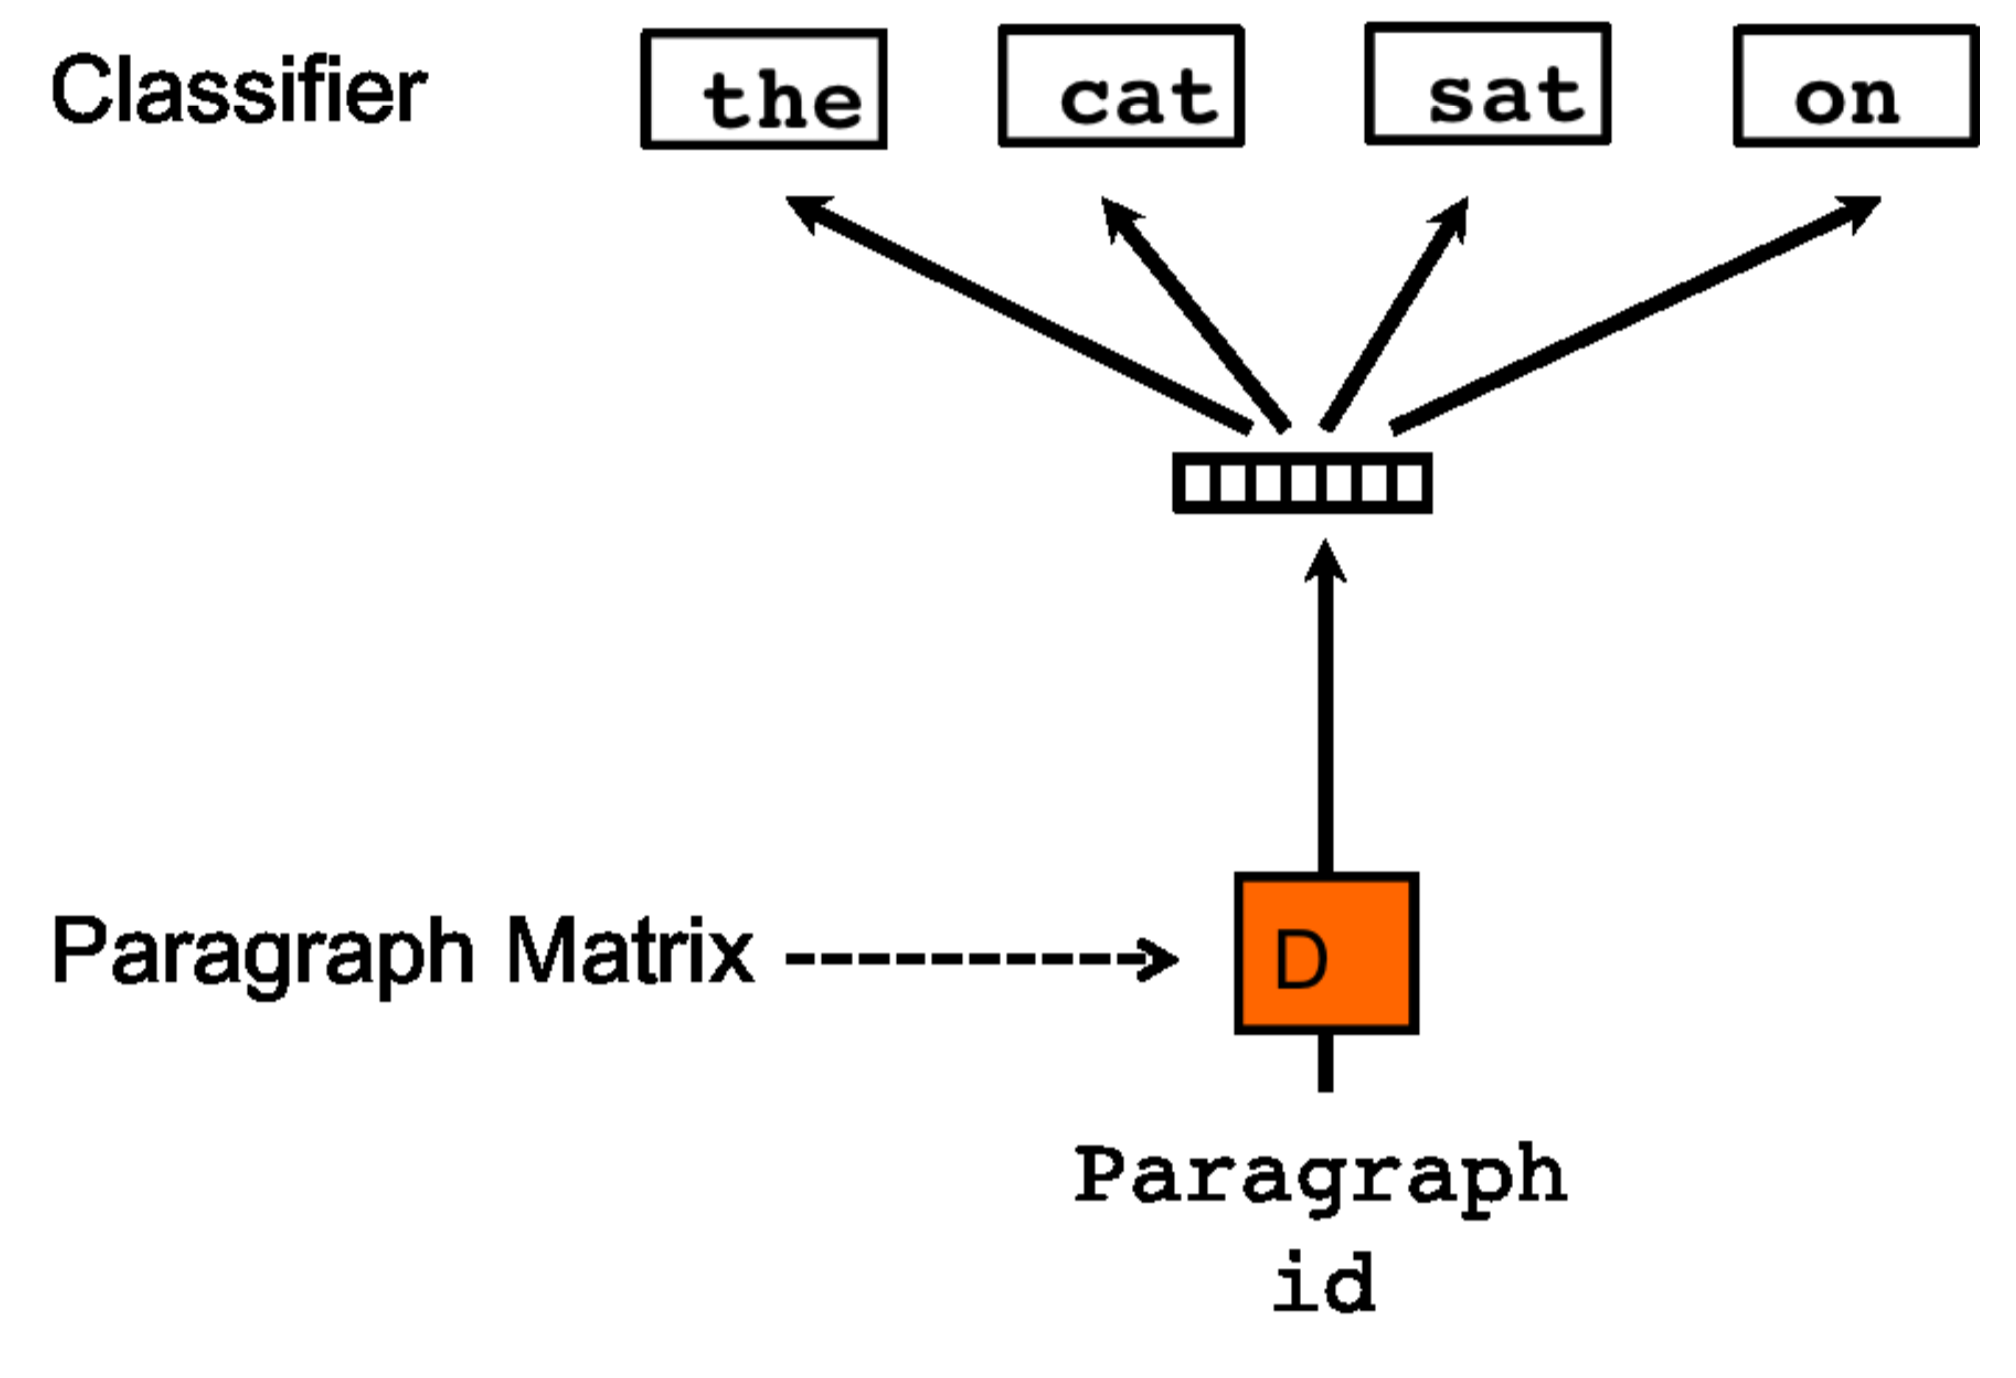
\includegraphics[width=0.6\textwidth]{figs/paragraph2vec.png}
\caption{Schematic of \textit{doc2vec} prediction taken from Le and Mikolov\cite{Le2014}. The document vector is used to predict words in a small window.}
\label{doc2vec}
\end{figure}


\subsection{Graph Embeddings or \textit{graph2vec}}

The problem statement here follows precisely the statement in the \textit{graph2vec} paper \cite{Narayanan} (Section 2). We give the intuition here. For a given graph $G = (N, E, \lambda)$, a rooted subgraph of degree $k$ around node $n \in N$ includes all the nodes and edges that are reachable in $k$ hops from $n$, see Fig \ref{fig:tree}. These rooted subgraphs $sg$ make up a graph $G$ in the same way that words make up a sentence. Our negative sampling objective then looks like:

$$
\arg\max_\theta
\sum_{(sg, G) \in \mathcal{D}}
    \log \dfrac{1}{1 + \exp{(-v_{sg} \cdot v_G)}}
+ \sum_{(sg, G) \in \mathcal{D^\prime}}
    \log \dfrac{1}{1 + \exp{(v_{sg} \cdot v_G)}}
$$

These subgraphs capture nonlinear structure in graphical data that linear paths, for example, do not \cite{SchweitzerPASCAL2011}. Subgraphs depend on the labels of the nodes and edges. In the results outlined in this paper, node labels were ignored (in our case, elements of the molecule), and instead nodes were by default labeled by their connectivity.\footnote{This was due to an unintentional technical mishap, but ended up providing a very interesting baseline regardless.}

\begin{figure}
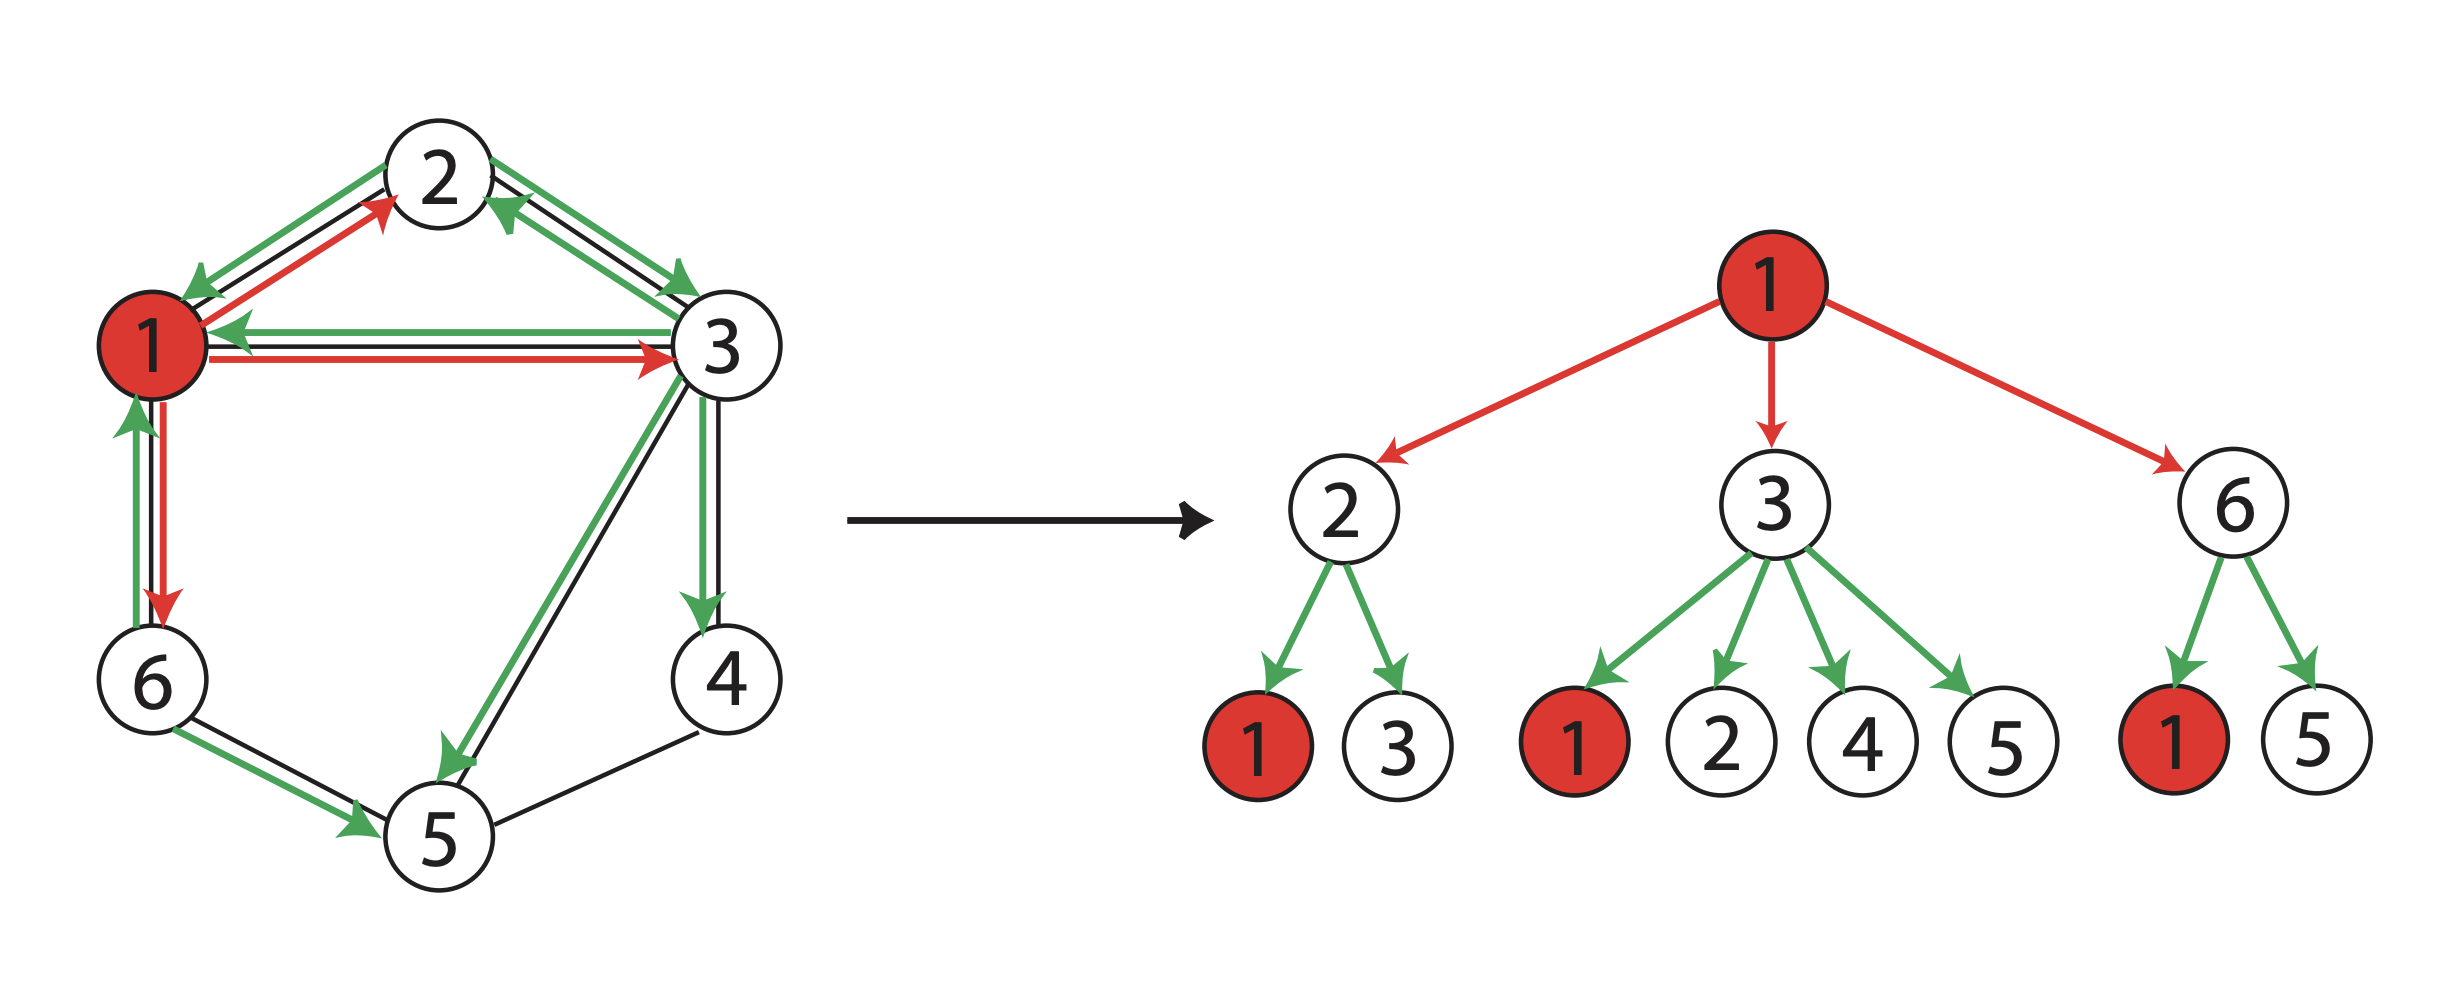
\includegraphics[width=\textwidth]{figs/tree_height_2.png}
\caption{Schematic showing the nodes reachable within two hops of the root node 1. Figure taken from Schweitzer and Pascal \cite{SchweitzerPASCAL2011}.}
\label{fig:tree}
\end{figure}
